\documentclass[a4paper,10pt]{report}
\usepackage[utf8]{inputenc}
\usepackage{graphicx}
\usepackage{verbatim}
\usepackage{ctable} % for \specialrule command

%\usepackage[a4paper, total={6in, 8in}]{geometry}
% Title Page
\title{\textbf{OPTICAL COMMUNICATION COMPONENTS \\ Laboratory Experiments}}
\author{Eridia Bozzetti\\Riccardo Fona\\Tigist Getachew\\Getahune Kebede\\Andrea Migliorati\\Davide Rocco\\Nicola Simoni\\Melkamsew Tenaw}
\date{University of Brescia, Faculty of Engineering\\A.Y. 2013-2014}


\begin{document}
\maketitle


%%%%%%%%%%%%%%%%%%%%%%%%%%%%%%%%%%%%%%%%%%%%%%%%%%%%%%%%%%%%%%%%%%%%%%%%%%%%%%%%%%%%%%%%%%%%%
\section*{Setup 1}
We measure the transmitted power by inserting an optical power meter between the laser and the multiplexer.\\
In Table \ref{powermeasures} are reported the power measures.

\begin{table}[ht!]
  \begin{center}
    \begin{tabular}{|c|c|c|}
      \specialrule{.1em}{.05em}{.05em}
	 $\lambda$ [nm] & Power [dBm] & Power [mW] \\
	\hline
	1550 & -2.97 & 0.5\\
	\hline
	1310 & -6.60 & 0.22\\
      \specialrule{.1em}{.05em}{.05em}
    \end{tabular}
  \end{center}
\caption{Power measures.}
\label{powermeasures}
\label{tab}
\end{table}


%%%%%%%%%%%%%%%%%%%%%%%%%%%%%%%%%%%%%%%%%%%%%%%%%%%%%%%%%%%%%%%%%%%%%%%%%%%%%%%%%%%%%%%%%%%%%
\section*{Setup 2}
The maximum laser output power of the optical power meter is 10 dBm. To avoid link damage we apply an attenuation of 6 dB,
so the effective output power is 4 dBm.

\subsection*{Method 1}
The laser wavelength is $\lambda=1552.52$ nm.
We first compute the attenuation due to the connectors, the insertion loss,
connecting only the pigtails fibers, obtaining a received power of:\\\\
\centerline{$P_{rx} = 2.61 $ $dBm$}\\\\
from this value is trivial to compute the insertion loss:\\\\
\centerline{$\alpha_{ins} = 4 - 2.61 = 1.39 $ $dB$}\\\\
Then we connect the link A and we measure the received power:\\\\ 
\centerline{$P_{rx_{link}} = -1.3 $ $dBm$}\\\\
the total attenuation is:\\\\
\centerline{$\alpha_{tot} = 4 - (-1.3) = 5.3 $ $dB$}\\\\
subtracting to it the insertion loss we obtain the attenuation of our link:\\\\
\centerline{$\alpha_{link} = 5.3 - 1.39 = 3.91 $ $dB$}\\\\

\subsection*{Method 2}
In this case our input is the Node A instead of the laser of the power meter as in the previous case.
For this measurement we have inserted optical coupler of $70\%-30\%$ power divider.
The measured power at the receiver, for the 1550 nm link, is:\\\\
\centerline{ $P=-19.67$ $dBm$}\\\\
Note that we measure only the $30 \%$ of the total power.\\
We first convert the measured values in linear scale, then we compute the total transmitted and received power:\\\\
\centerline{ $P_{tx}=0.50 \cdot \frac{100}{30} = 1.67$ $mW$}\\\\
\centerline{ $P_{rx}=0.011 \cdot \frac{100}{30} = 0.37$ $mW$}\\\\
that in logarithmic scale are:\\\\
\centerline{ $P_{tx_{dBm}}= 2.23$ $dBm$}\\\\
\centerline{ $P_{rx_{dBm}} = -4.32$ $dBm$}\\\\
We can now compute again the total attenuation:\\\\
\centerline{$\alpha_{tot} = 2.23 - (-4.32) = 6.55 $ $dB$}\\\\
finally, subtracting the insertion loss computed earlier, we obtain the fol\-lowing link attenuation value:\\\\
\centerline{$\alpha_{link} = 6.55 - 1.39 = 5.16 $ $dB$}\\\\

The difference between the values of the two methods is due to the different number of connectors, that modify the
insertion losses, and to the uncertainty of the measurements.

\newpage
\section*{Setup 3}
We measure the throughput of the 1310 nm link as a function of the attenuation.\\
In the Figure \ref{throughput} are reported the measured values:
we observe that the throughput is almost constant until an attenuation of 9 dB, then it immediately falls.


\begin{figure}[!ht]
   \centering
   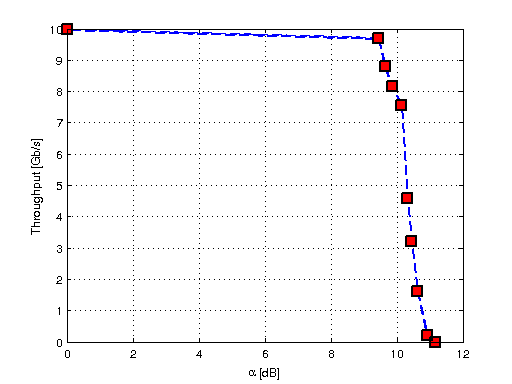
\includegraphics[width=12cm]{throughput.png}\\
   \caption{Throughput versus attenuation.}
   \label{throughput}
\end{figure}

\end{document}